\documentclass{article}

% Language setting
% Replace `english' with e.g. `spanish' to change the document language
\usepackage[english]{babel}

% Set page size and margins
% Replace `letterpaper' with `a4paper' for UK/EU standard size
\usepackage[letterpaper,top=2cm,bottom=2cm,left=3cm,right=3cm,marginparwidth=1.75cm]{geometry}

% Useful packages
\usepackage{amsmath}
\usepackage{float}
\usepackage{graphicx}
\usepackage[colorlinks=true, allcolors=blue]{hyperref}

\title{Računalniška grafika zapiski}
\author{Tim Hajdinjak}

\begin{document}
\maketitle

\section{Matematične osnove}

Osnovni pojmi, brez katerih žal ne gre

\begin{itemize}
\item stolpčna matrika: $\begin{bmatrix} 2,9 \\ -4,6 \\ 0 \end{bmatrix}$
\item vrstična matrika:  $\begin{bmatrix} 12,5 & -9,32 & 0 \end{bmatrix}$
\item transponiranje: pomeni zamenjavo osi dveh matrik: $\begin{bmatrix} 1,3 & -4,1 & 0,0 \end{bmatrix}^T = \begin{bmatrix} 1,3 \\ -4,1 \\ 0,0 \end{bmatrix}$
\item enakost matrik: dve matriki sta si enaki, če imata enako število elementov po obeh oseh, in so vsi elementi na enakih mestih
\item vektor: predstavljen kot matrika, pomeni premik iz točke v točko in vektorji nimajo lokacije
\item seštevanje matrik: $a + b = c \iff c_i = a_i + b_i$, intuitivno: 
\begin{figure}[H]
\centering
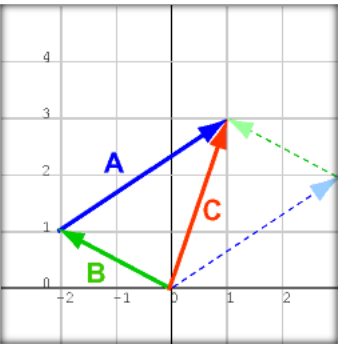
\includegraphics[width=25mm]{sestevanje_vektorjev.png}
\caption{Geometrijsko sestevanje vektorjev.}
\end{figure}
\end{itemize}

\section{Some examples to get started}

\subsection{How to create Sections and Subsections}

Simply use the section and subsection commands, as in this example document! With Overleaf, all the formatting and numbering is handled automatically according to the template you've chosen. If you're using the Visual Editor, you can also create new section and subsections via the buttons in the editor toolbar.

\subsection{How to include Figures}

First you have to upload the image file from your computer using the upload link in the file-tree menu. Then use the includegraphics command to include it in your document. Use the figure environment and the caption command to add a number and a caption to your figure. See the code for Figure \ref{fig:frog} in this section for an example.

Note that your figure will automatically be placed in the most appropriate place for it, given the surrounding text and taking into account other figures or tables that may be close by. You can find out more about adding images to your documents in this help article on \href{https://www.overleaf.com/learn/how-to/Including_images_on_Overleaf}{including images on Overleaf}.

\begin{figure}
\centering
\includegraphics[width=0.25\linewidth]{frog.jpg}
\caption{\label{fig:frog}This frog was uploaded via the file-tree menu.}
\end{figure}

\subsection{How to add Tables}

Use the table and tabular environments for basic tables --- see Table~\ref{tab:widgets}, for example. For more information, please see this help article on \href{https://www.overleaf.com/learn/latex/tables}{tables}. 

\begin{table}
\centering
\begin{tabular}{l|r}
Item & Quantity \\\hline
Widgets & 42 \\
Gadgets & 13
\end{tabular}
\caption{\label{tab:widgets}An example table.}
\end{table}

\subsection{How to add Comments and Track Changes}

Comments can be added to your project by highlighting some text and clicking ``Add comment'' in the top right of the editor pane. To view existing comments, click on the Review menu in the toolbar above. To reply to a comment, click on the Reply button in the lower right corner of the comment. You can close the Review pane by clicking its name on the toolbar when you're done reviewing for the time being.

Track changes are available on all our \href{https://www.overleaf.com/user/subscription/plans}{premium plans}, and can be toggled on or off using the option at the top of the Review pane. Track changes allow you to keep track of every change made to the document, along with the person making the change. 

\subsection{How to add Lists}

You can make lists with automatic numbering \dots

\begin{enumerate}
\item Like this,
\item and like this.
\end{enumerate}
\dots or bullet points \dots
\begin{itemize}
\item Like this,
\item and like this.
\end{itemize}

\end{document}